%&pdflatex
%
%  Comparison of Numerical Models for Coastal Dynamics - 1D Theory
%
%  Authors:
%
\documentclass[]{article}

\usepackage{graphicx}

% Use utf-8 encoding for foreign characters
\usepackage[utf8]{inputenc}

% Multipart figures
% \usepackage{subcaption}

% More symbols
\usepackage{amsmath}
\usepackage{amssymb}
\usepackage{latexsym}

% URL and linking help
\usepackage{hyperref}

% Package for including code in the document
\usepackage{listings}
% \DeclareCaptionFont{white}{\color{white}}
% \DeclareCaptionFormat{listing}{%
%   \parbox{\textwidth}{\colorbox{gray}{\parbox{\textwidth}{#1#2#3}}\vskip-4pt}}
% \captionsetup[lstlisting]{format=listing,labelfont=white,textfont=white}
% \lstset{frame=lrb,xleftmargin=\fboxsep,xrightmargin=-\fboxsep,numbers=left,basicstyle=\ttfamily\small,language=python,columns=fixed,commentstyle=\em\color[rgb]{0.133,0.545,0.133}}

% This is now the recommended way for checking for PDFLaTeX:
\usepackage{ifpdf}

% Add line numbers
\usepackage[mathlines]{lineno}

% Need to use this package to handle the spacing issues in LaTeX after a command
\usepackage{xspace}

% Markup
\usepackage{color}
\newcommand{\comment}[1]{\color{blue} #1}
\newcommand{\alert}[1]{\textbf{\color{red} #1}}

\graphicspath{{./figures/}}



% Useful commands
%!TEX root = paper.tex
%  Generic math macros
\renewcommand{\v}[1]{\boldsymbol{#1}}
\newcommand{\m}[1]{\text{\textsf#1}}

\newcommand{\pd}[2]{\ensuremath{\frac{\partial #1}{\partial #2}}} % partial
\newcommand{\dee}{\ensuremath{\mathrm{d}}}                  % d symbol
\newcommand{\diff}[2]{\ensuremath{\frac{\dee #1}{\dee #2}}} % Derivative d/dx
% \newcommand{\grad}{\ensuremath{\nabla}}                     % Gradient symbol
\newcommand{\gradient}{\ensuremath{\textsf{grad}}}          % Written gradient
\newcommand{\Div}{\ensuremath{\nabla \cdot}}                % Divergence
\newcommand{\divergence}{\ensuremath{\textsf{div}}}         % Written div
\newcommand{\del}{\ensuremath{\nabla}}                      % Same as gradient
\newcommand{\delsq}{\ensuremath{\nabla^2}}                  % Laplacian
\newcommand{\lap}{\ensuremath{\delsq}}                      % Laplacian
\newcommand{\dx}{\ensuremath{\Delta x}}                     % Delta x
\newcommand{\dy}{\ensuremath{\Delta y}}                     % Delta y
\newcommand{\dt}{\ensuremath{\Delta t}}                     % Delta t
\newcommand{\scinot}[2]{\ensuremath{#1\times10^{#2}}}       % Scientific note
\newcommand{\bigO}[1]{\ensuremath{\mathcal{O}(#1)}}         % Big O notation
\newcommand{\R}{\ensuremath{\mathbb{R}}}                    % Real field
\newcommand{\Z}{\ensuremath{\mathbb{Z}}}                    % Integer field
\newcommand{\half}{\ensuremath{\frac{1}{2}}}                % 1/2 fraction

%  Special formatting for codes
\newcommand{\geoclaw}{{\sc GeoClaw}\xspace}
\newcommand{\clawpack}{{\sc Clawpack}\xspace}
\newcommand{\amrclaw}{{\sc AMRClaw}\xspace}
\newcommand{\pyclaw}{{\sc PyClaw}\xspace}
\newcommand{\forestclaw}{Forestclaw\xspace}

%  Finite volume method symbols
\newcommand{\wave}{\ensuremath{\mathcal{W}}\xspace}             % Wave
\newcommand{\fwave}{\ensuremath{\mathcal{Z}}\xspace}            % F-Waves
\newcommand{\cell}{\ensuremath{\mathcal{C}}\xspace}             % FV grid cell
\newcommand{\apdq}{\ensuremath{\mathcal{A}^+ \Delta Q}\xspace}      % A+dq
\newcommand{\amdq}{\ensuremath{\mathcal{A}^- \Delta Q}\xspace}      % A-dq
\newcommand{\apmdq}{\ensuremath{\mathcal{A}^{\pm} \Delta Q}\xspace} % A+-dq

% B+-A+-dq symbols
\newcommand{\BpApdq}{\ensuremath{\mathcal{B}^{+} \mathcal{A}^{+} \Delta Q}\xspace}
\newcommand{\BpAmdq}{\ensuremath{\mathcal{B}^{+} \mathcal{A}^{-} \Delta Q}\xspace}
\newcommand{\BmApdq}{\ensuremath{\mathcal{B}^{-} \mathcal{A}^{+} \Delta Q}\xspace}
\newcommand{\BmAmdq}{\ensuremath{\mathcal{B}^{-} \mathcal{A}^{-} \Delta Q}\xspace}
\newcommand{\BpmApmdq}{\ensuremath{\mathcal{B}^{\pm} \mathcal{A}^{\pm} \Delta Q}\xspace}

% commands for nonhydrostatic part
\newcommand\Bt{Boussinesq-type}
\newcommand\Bte{\Bt\ equations}
\newcommand\da{depth-averaged}
\newcommand\nh{nonhydrostatic}
\newcommand\Nh{Nonhydrostatic}
\newcommand\nheswe{\nh\ extension for shallow water equations}
\newcommand\danheswe{\da\ \nheswe}
\newcommand\nhp{\nh\ pressure}
\newcommand\fnh{f_{\text{nh}}}
\newcommand\fgn{f_{\text{d}}}
\newcommand\bu{\boldsymbol{u}}
\newcommand\bU{\boldsymbol{U}}
\newcommand\bx{\boldsymbol{x}}
\newcommand\csw{c_{\text{sw}}}
\newcommand\Pnh{P^{nh}}
\newcommand\Pnhd{P^{nh}_{-d}}
\newcommand\pnh{p^{nh}}
\newcommand\bnabla{\boldsymbol{\nabla}}




\begin{document}

\ifpdf
\DeclareGraphicsExtensions{.pdf, .png, .jpg, .tif}
\else
\DeclareGraphicsExtensions{.png, .jpg, .tif, .eps}
\fi

\title{Comparison of Numerical Models for Coastal Dynamics}

\author{Kyle T. Mandli\thanks{
            Columbia University} \and
        Nishant Panda\thanks{
            Colorado State University} \and
        Anja Jeschke\thanks{
            University of Hamburg}
        }

\maketitle

\begin{abstract}
    Put really awesome abstract here.
\end{abstract}

\begin{itemize}
    \item Theoretical Paper
    \begin{enumerate}
        \item Intro to different PDE systems being considered
        \item Dispersion analysis
        \item 1D tests
        \item status
        \begin{enumerate}
            \item KdV (Panda)
            \item Serre-Green-Naghdi (Panda)
            \item Boussinesq-Green-Naghdi (Panda)
            \item Shallow water (Mandli)
            \item 2-layer shallow water (Mandli)
            \item Nonhydrostatic extension for shallow water equations (Jeschke)
        \end{enumerate}
    \end{enumerate}
\end{itemize}



\begin{tabular}{c|ccccc}
\textbf{Model} & Well-balanced & Inundation & 2D & Non-Hydrostatic & Linear Dispersion \\
\hline \hline
SWE                     & yes & yes & yes &  no &  ~  \\
Serre-Green-Naghdi      &  ~  &  ~  &  ~  &  ~  &  ~  \\
Boussinesq-Green-Naghdi &  ~  &  ~  &  ~  &  ~  &  ~  \\
Non-Linear KdV          &  ~  &  ~  &  ~  &  ~  &  ~  \\
2-Layer SWE             & yes & yes & yes &  no &  ~  \\
Non-hydrostatic         & yes & ca. & yes & yes &  ~  \\
\end{tabular}

\section{Introduction}

\subsection{Selection Criteria}
\begin{itemize}
    \item Limit models to those that have the following properties:
    \begin{itemize}
        \item Well-balanced
        \item Handles inundation?
        \item 2D or at the most semi-3D (layers) - this may troublesome to differentiate as most hydrostatic ocean codes are really layered 3D models
    \end{itemize}
\end{itemize}

\section{Models} 

%!TEX root = paper.tex
\subsection{Depth-averaged \nheswe}
The \nheswe\ is linked to the solution of the Euler equations using kinematic boundary conditions on the surface and the bottom. The basis of the method is a projection method (see e.g. \cite{Chorin.1968}) solving the time-discretized equations stepwise. 
The pressure is decomposed into a hydrostatic and a \nh\ part \cite{CasulliStelling.1998, StansbyZhou.1998}. This splitting has the advantage that the solver for the \nh\ equations can resort to the solver for the shallow water equations. 
The \da\ version of this apporach was derived from a multi-layer formulation  \cite{StellingZijlema.2003} applying linear approximations between different layers, s.t. also the \nhp\ is assumed to be linear in the multi-layer equations. On the other hand, the vertical Euler equation leads to a quadratic vertical profile of the \nhp when considering \da\ equations. Therefore, there are two possibilities to choose the pressure profile.
Under the assumption of small vertical variations of horizontal velocities, the \danheswe\ is derived out of the Euler equations for \da\ variables
\begin{align}
  (u,v)=\bu:=\frac{1}{h}\int_{-d}^{\xi}{\bU}\,dz, \qquad w:=\frac{1}{h}\int_{-d}^{\xi}{W}\,dz, \qquad \pnh&:=\frac{1}{h}\int_{-d}^{\xi}{\Pnh}\,dz. \label{eq:def_pnh}
\end{align}
The \danheswe\ is described with the equation system
\begin{align}
\partial_t \xi+\bnabla \cdot (h\bu)=&0, \label{eq:nh_conti} \\
\partial_t \bu+(\bu \cdot \bnabla)\bu=&-g\bnabla \xi-\frac{1}{\rho h}\left(\bnabla \left(hp^{nh} \right) -\fnh\pnh \bnabla d\right), \label{eq:nh_Momxy} \\
\partial_t w+(\bu \cdot \bnabla)w=&\frac{1}{\rho h}\fnh\pnh, \label{eq:nh_Momz} \\
2 \left(w+\bu \cdot \bnabla d \right)=&-h\left(\bnabla \cdot \bu\right), \label{eq:nh_closure}
\end{align} 
where the scalar $\fnh$ refers to the chosen pressure profile. In case of the linear pressure profile
\begin{equation}
  P^{nh}(z)=\frac{\Pnhd}{h}(\xi -z),
\end{equation}
with $\Pnhd$ being the \nhp\ at the bottom, it is $\fnh=2$, whereas it is $\fnh=1.5$ in the case of the quadratic pressure profile
\begin{equation}
 P^{nh}(z)=\frac{1}{2}\frac{\Gamma}{h}\left(-(z+d)^2+h^2\right)%+\rho\Phi\left(\xi-z\right) \label{eq:Pnh_quadr_z}
\end{equation}
with
\begin{align*}
  \Gamma &:= \rho h\left( -(\bnabla \cdot \partial_t \bu) - (\bu \cdot \bnabla) (\bnabla \cdot \bu) + (\bnabla \cdot \bu)^2 \right). \\
  %\Phi &:= - \bnabla d \cdot \left( \partial_t  \bu + (\bu \cdot \bnabla)\bu \right) - \bu \cdot \bnabla(\bnabla d) \cdot \bu.
\end{align*}
For a more detailed derivation see \cite{Jeschke.2016}.


The spatial discretization of the shallow water equations implements the $P^{NC}_1$--$P_1$ finite element method as described in \cite{Hanert.2005, LeRouxPouliot.2008} with the $P^{NC}_1$--$P_1$ advection scheme of \cite{Androsov.2011}. It uses nonconforming linear basis functions for the horizontal velocities and conforming linear basis functions for the height. A two-dimensional computational domain is represented by a structured triangulation generated with the adaptive mesh generator amatos \cite{Behrens.2005}. The time-stepping scheme applies the Leapfrog method stabilized with the Robert-Asselin filter \cite{Asselin.1972} using $\alpha=0.025$.

The \danheswe\ \eqref{eq:nh_conti}--\eqref{eq:nh_Momz} is solved based on the projection method proposed in \cite{StellingZijlema.2003}. The advantage of this method is that the shallow water solver does not have to change in order to solve the \nh\ equation system. This projection method involves the solution of a Poisson equation for the \nhp\ in each timestep, which is constructed as follows: The time-discretized horizontal momentum equations are written as an intermediate solution in the present timestep plus a correction term depending on the \nhp. Together with the time-discretized vertical momentum equation, this splitting is substituted into equation \eqref{eq:nh_closure} in its weak formulation to receive the Poisson equation. The emerging linear equation system is solved by means of a GMRES algorithm. The computed \nhp\ is added to the intermediate horizontal velocities and to the vertical velocity of the previous time step. At this point, the velocities have been updated and the numerical solution of the continuity equation completes the computation of the timestep.
To discretize the \nhp\ and vertical velocity, conforming linear basis functions are used. The same approach was taken in \cite{Fuchs.2013}, but we retain an absent bathymetry gradient term. 

\section{Dispersion Analysis} \label{sec:dispersion}

\section{Benchmarks}

\begin{itemize}
    \item \url{https://github.com/rjleveque/nthmp-benchmark-problems}
    \item \url{https://github.com/rjleveque/geoclaw-group/tree/master/benchmarks}
    \item \url{https://github.com/rjleveque/tsunami_benchmarks}
    \item \url{http://depts.washington.edu/clawpack/geoclaw/benchmarks/nthmp_currents_2015/}
\end{itemize}

\begin{tabular}{c|cccc}
\textbf{Dimensionality} & \textbf{Benchmark} & Analytical & Experimental & Field \\
\hline \hline
1D & Solitary Wave on a Simple Beach    & X          & X & ~ \\
~  & Solitary Wave on a Composite Beach & X (linear) & X & ~ \\
~  & Solitary Wave translating          & X          & X & ~ \\
~  & Trapezoidal Berm                   & ~          & X & ~ \\
\end{tabular}

\subsection{Linear standing wave}
The linear standing wave test illustrates the different linear dispersion relations and the ability of the numerical method to represent them in an accurate manner. 
Both, the linearized systems of the hydrostatic and dispersive have an analytic standing wave solution
\begin{align}
\xi(\bx,t)&=-a\sin\left(\kappa x \right)\cos\left(\kappa ct\right), \\
 u(\bx,t) &=a \frac{c}{d}\cos\left(\kappa x\right)\sin\left(\kappa ct\right), \\
 v(\bx,t) &=0, \qquad \forall \ \bx=(x, y)^T \in \Omega, \forall t \in \mathbb{R},
\end{align}
where the phase velocity $c=\frac{\omega_{\text{nh,}\fnh}}{\kappa}$ is chosen for the dispersive equation set and $c=\csw$ for the hydrostatic equation set, respectively. For the \nh\ model, the analytic vertical velocity has to be defined as
\[
w(\bx,t)=-\frac{d}{2}\partial_x u=\frac{1}{2}ac\kappa\sin\left(\kappa x \right)\sin\left(\kappa ct\right),
\]
which is derived directly from \eqref{eq:nh_closure}.
In different model runs, we vary the depth $d$ while keeping the wave length $\lambda=\frac{2\pi}{\kappa}=20$ m and the amplitude $a=0.01$m constant to get ratios for $\frac{d}{\lambda}$ between $0.05$ and $1.0$, and ratios for $\frac{a}{d}$ between $0.01$ and $0.005$, respectively.
We impose double periodic boundary conditions on a grid length of one wave length. The simulation time is chosen long enough to measure one wave period. 

\subsubsection{Results of \nh\ model}
The resulting normalized phase velocities for the shallow water model and the \nh\ equation set with either the linear or the quadratic vertical pressure are displayed in figure \ref{fig:nh_standingwave}. Furthermore, they are compared to their analytical reference phase velocities and the full reference phase velocity as derived in section \ref{sec:dispersion}. 
In each case, the numerical dispersion relation matches the corresponding analytical one precisely.
% The coincidence between numerical and analytical phase velocities is very good. 
In a close neighborhood of the shallow water assumption (i.e., in the limit $\frac{d}{\lambda} \rightarrow 0$), the quadratic vertical pressure profile gives a better phase velocity compared to the full reference solution than the linear profile, as expected from series expansions around this state used in \Bt\ models.
% \svnote{Can we have an additional detail plot of this neighborhood?} \ajnote{Then only thinner lines would help. I could also provide the whole image with different plotting style (thinner lines and ) One could also use absolute errors between numerical values and reference phase velocities. }\jbnote{What are you expecting to see?}\svnote{I expect to see what we describe in the text, i.e., that the quadratic vertical pressure profile gives a better phase velocity than the linear one near $d/\lambda=0$, see added figure.}
However, for ratios $\frac{d}{\lambda} > 0.25$ approximately, the linear profile matches better.

\begin{figure}[htbp]
        \includegraphics*[width=0.95\textwidth]{nh_standingwave.eps}
        \caption{Standing wave: Comparison of simulated hydrostatic and \nh\ phase velocities with analytic reference values for all simulations (left) and a zoom onto the close neighborhood of the long wave limit (right)}
        \label{fig:nh_standingwave}
\end{figure}


\subsection{Propagating solitary wave}
The propagating solitary wave tests the balancing of dispersion effects and nonlinearity for an appropriate initial condition.
On constant bathymetry, the Serre equations \cite{Serre.1953} have an analytic solitary wave solution
\begin{align}
\label{eq:Serre_sol_surface}
\xi(\bx,t)&=a \ \text{cosh}^{-2}(K(x-ct-x_0)), \\
u(\bx,t)&=c\frac{\xi(\bx,t)}{d+\xi(\bx,t)},
\end{align}
with the ratio $\frac{a}{d}=0.2$, propagation velocity $c=\sqrt{g(d+a)}$ on a constant depth $d=10 \, \text{m}$, scale factor $K=\sqrt{\left(\frac{3a}{4d^2(d+a)}\right)}$ and displacement $x_0=l/2$ on a domain of length $l=800 \, \text{m}$.
Again, we impose double periodic boundary conditions solitary wave propagating in the positive $x$-direction. The simulation time is $30$ seconds.

\subsubsection{Results of \nh\ model}
The equations \eqref{eq:nh_conti}--\eqref{eq:nh_closure} using the quadratic vertical pressure profile are equivalent to the Serre equations \cite{Serre.1953}, which is shown in  \cite{Jeschke.2016}. Using the linear vertical pressure profile, there is no equivalence to the Serre equations.
For the \nh\ model, we also need to initialize the vertical velocity, which directly follows from equation Equation \eqref{eq:nh_closure}, s.t.
\begin{align}
w&=-0.5h\partial_x u. \label{eq:nh_solit_init_w}
\end{align}
Figure \ref{fig:nh_solitarywave} compares our numerical computations with the analytical solution at the end of the simulation time.
The numerical result using the quadratic pressure profile shows a very good agreement with the analytical solution. In contrast, the application of the linear pressure profile yields a threefold mismatch arising from the inconsistency in initial conditions combined with the underlying equation system: Small amplitude waves propagate to the opposite direction, the wave height increases {because of weaker dispersion of the linear profile and trailing waves start to establish.
In \cite{StellingZijlema.2003, Walters.2005, Yamazaki.2008}, different solitary waves are computed with \nh\ models using the traditional linear vertical pressure profile. Therein, these mismatches are also visible, except that their amplitudes tend to diminish than to amplify. The reason is the application of another vertical velocity, namely $W(z)=-z\partial_x u$, so $w=-0.5(\xi-d)\partial_x u$. If the term $-d\partial_x u$ is added, the vertical velocity \eqref{eq:nh_solit_init_w} results. Hence, in \cite{StellingZijlema.2003, Walters.2005, Yamazaki.2008}, the vertical velocity is too large on the left hand side of the maximum amplitude and too small on the right hand side, which decreases the nonlinear steepening of the wave.
Their aim to compute the solitary waves was merely to show that \nh\ models produce similar results as \Bt\ models. 

\begin{figure}[htbp]
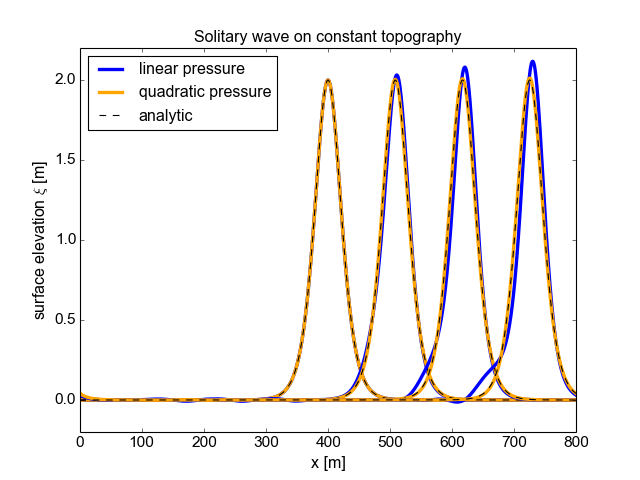
\includegraphics[width=\textwidth]{nh_solitary}
\caption{Comparison of the analytical (black) sea surface height of the
solitary wave with the simulation results of the quadratic (yellow) and linear (blue) vertical profile after a propagation time of 10, 20 and 30 seconds to the right.}
\label{fig:nh_solitarywave}
\end{figure}


\begin{flushleft}
    \bibliographystyle{abbrv}
    \bibliography{references}
    \addcontentsline{toc}{section}{References}
\end{flushleft}

\end{document}
